\documentclass[]{article}
\usepackage{indentfirst, graphicx, caption, subfigure}
\usepackage[margin=1in]{geometry}
\usepackage[T1]{fontenc}
\setlength\parindent{0pt}
\begin{document}

\title{ASTR W3646 \\ Observational Astronomy \\ Final Project \\ Computer Vision Experiments in Crowdsourced Astronomy}
\author{Rasmi Elasmar}
\date{Monday, December 21, 2015}
\maketitle
\section*{Introduction}
The contributions of amateur observers and citizen scientists in astronomy have become more meaningful in doing "real science" through both crowdsourced data analysis and telescope observations (Marshall 2015). There remains huge untapped potential in crowdsourcing amateur observations on the internet and extracting meaningful scientific data from them. Some laborious attempts tailored towards particular objects (e.g. comets) have proven successful (Lang 2012), but there remains work to be done in generalizing the crowdsourcing process and improving the way data is retrieved and consolidated. This project seeks to mine and process images from AstroBin, a website where amateur and professional astronomers can post their observations. AstroBin is likely to provide images of a higher quality and with more accurate metadata than more generalized web searches because of its user base. The API, which is liberal in its terms of use, allows for searching by object, date, and by telescope properties, which can allow for interesting applications in analyzing the data. 
\\\\
This project explores methods of processing images of varying quality and content in hopes of creating time-series visualizations of Solar System objects such as the Moon and Jupiter. This turned out to be a much greater challenge than was initially suspected; however, progress was made and lessons were learned throughout the process.
\section*{Process}
\subsection*{Data Gathering}
AstroBin provides a searchable API. Images can be tagged by Solar System object upon submission, but this isn't guaranteed and may exclude results. To ensure thoroughness, run two searches: one with "jupiter" in the title, and one for "jupiter" in the description. On 12/18/15, these returned 7,532 and 2,047 results, respectively, for a total of 9,579 results. After removing duplicates by ID, 7,875 images remain. Once the IDs and metadata are in place, downloading the images is a simple but time-consuming and storage-intensive process.
\\\\
On the first attempt, 7,867 images were downloaded and 8 failed. After a second attempt, 5 more images downloaded and 3 failed again, for a total of 7,872 images. Subsequent attempts yielded no new images.
\\\\
Running similar searches for "Moon" on 12/19/15 returned 9,551 and 4,812 results, respectively, for a total of 14,363 results. After removing duplicates by ID, 12,152 images remain. Two image downloads continued to fail after multiple attempts, leaving a total of 12,150 images.
\subsection*{Data Cleansing}
A cursory look through the downloads yields images of highly variable quality. We consider approaches to cleaning our data to move forward in time series analysis. Not all images contain Jupiter or the Moon in detail. For example, some may be of the entire night sky, in which Jupiter may only appear as a small dot. Other images may be excessively blurry or out of focus. Some images contain two or more pictures of our desired object which have been arranged side-by side. Additional concerns include annotations and other post-processed effects. Some images are not even of the planet Jupiter (our search returned multiple results for NGC 3242, the Ghost of Jupiter nebula), or Earth's Moon in particular.
\\\\
We would ideally keep only the highest-quality images available to us. We must also consider alignment of our object within the images, which tends towards the center but generally varies. We don?t want to exclude zoomed-out images that may contain Jupiter?s Moons or other transient phenomena. We can judge these qualities visually by detail, sharpness, clarity, and so on; however, to judge many thousands of images visually is infeasible given time constraints and the scale of images available on the Internet.
\\\\
We would like an approach that can classify these images for us. Judging from the metadata, we can group images by author, which may give us images which are visually similar (taken with the same equipment, and perhaps around the same time). We can also sort images by upload time and cluster images which were uploaded together to also potentially group similar images. While these are all useful approaches, metadata is ultimately untrustworthy and can only give us so much information. Using computer vision to perform visual classification is far more powerful and flexible when it comes to deciding which images we should ultimately keep and analyze.
\section*{Computer Vision Methods}
There are a variety of approaches that can be taken in using computer vision to decide which images we should keep and extracting information from those images. Computers are excellent at pattern searching and matching for well-defined patterns. For example, removing images which do not contain Jupiter can be done by defining a template of Jupiter and searching the images for that template. Classifiers can also be trained to group images based on a training set of data (of various planets, for example). 
\\\\
We could also combine images based on similarity to other images. For example, if two images contain Jupiter's Great Red Spot, they are likely to cover a similar portion of Jupiter. Using this approach, we can "wrap" around the planet by clustering images starting from a single point and rotating from that point to images which are similar. This can easily be made inefficient given the wrong approach. Jupiter's complex but not entirely unique features make it difficult to do in-depth pattern matching quickly and on a large scale.
\\\\
In the interest of simplicity, we focus solely on the Moon data. The Moon presents a nice challenge: given images of the Moon, can we guess its phase? Looking at histograms of Moon images suggest that it may be possible to distinguish the phase of the Moon by the distribution of the pixel values. There are multiple thresholding methods that can help us decide how much of the Moon is illuminated, and classification and pattern-matching may also be of use.
\\\\
If we can accurately guess its phase, combined with upload date sorting to group images by approximate date taken or uploaded from the metadata (so as to not combine similar Moon phases from different months together), these computer vision methods may provide us with an effective approach.
\subsection*{Thresholding and Segmentation Methods}
Thresholding methods seek to distinguish areas of interest from areas of non-interest. In this case, we are interested in the illuminated portions of the Moon and not in the sky or the dark portions of the Moon. The illuminated portions of the Moon (and our images) provide an excellent proxy for its current phase.
\\\\
We can try using Otsu's method to split the image into illuminated Moon parts and dark sky/non-illuminated Moon parts. Otsu's method operates by choosing an ideal threshold in a bimodally distributed image's histogram which turns the image into a binary white/black image. Because images of the Moon contain dark and light portions, once the image is reduced to its binary form, we can take a proportion of illuminated pixels to judge which phase the Moon is in. This can be affected by background objects or by the crop of the image (for example, if an image is zoomed in to only capture an illuminated crescent, it will register a higher illuminated proportion than a zoomed-out image of the Moon showing a small crescent), so ideally we would identify the Moon and limit our proportion calculation to a circular area. A simpler version of this method would just compute some normalized cutoff based on the histogram's dropoff, but this can be noisy if the Moon and background share colors.
\\\\
We can also use the Canny edge detector to detect the edge of the Moon against the background of the sky. Filling the borders of these edges would yield the desired result. This may also allow us more precision in outlining the exactly illuminated chunk of the Moon, moving precisely along the lunar terminator. Again, calculating some proportion of filled vs. non-filled parts of the image would reveal the phase of the Moon.
\\\\
Similarly, we can use region-based segmentation to select only the illuminated portion of the Moon. Region-based segmentation works by defining some area of interest and non-interest (the illuminated Moon vs. the dark sky) and filling outwards from those areas of interest until we reach some gradient dropoff into an area of non-interest. This is a neat and reliable method given the right data, but computationally selecting foreground and background samples in an image at large scales may be difficult or unreliable. We could select the darkest portion of the histogram as the are of non-interest and the brightest as the area of interest, and this should generally work for images of only the Moon, but for images  that contain other objects, we may receive mixed results.
\subsection*{Templates and Classification}
Alternatively, we can train a classifier for all different phases of the Moon and run it on all the images. This is the most scalable approach, but requires a usable training dataset for supervised learning. A classifier may also fail easily if the image is not mostly focused on the Moon, unless it was trained with similarly noisy or unfocused data. Because the quality of our images varies siginificantly, we would need a large training set to reliably sort through these thousands of images.
\\\\
Template-based classification requires no training. Using the scikit-image Python library, we can define a template and search for occurrences in an image which match that template. This method is based on the cross-correlation of the template and target image (Briechle and Hanebeck 2001; J. P. Lewis 1995). We can create templates for each phase of the Moon and search each image for all possible phases of the Moon, selecting the template with the highest correlation. This requires more computational power than a classifier because we brute-force search each image as many times as we have templates, but it may be easier to implement. It also can identify occurrences of the Moon in images which do not explicitly focus on the Moon, which may be helpful given our diverse dataset.
\pagebreak
\section*{Analysis}
\subsection*{Results}
We analyze the results of the approaches described above when applied to a single sample image (Figure 1).
\begin{figure}[h]
\centering
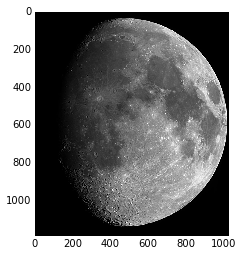
\includegraphics{sample_moon}
\caption{A sample image of the Moon from AstroBin.}
\end{figure}
\subsubsection*{Simple Filtering}
We can take a look at the histogram (Figure 2) of the image to get an idea of the pixel distribution (from 0 to 1) of the grayscale image.
\begin{figure}[h]
\centering
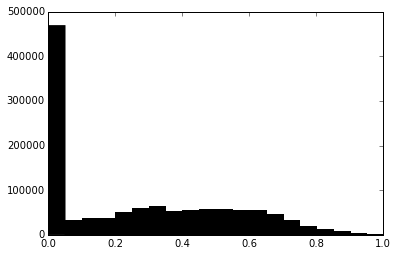
\includegraphics[scale=0.6]{hist}
\caption{Histogram of grayscale pixel values of the sample image. Bin size was increased  to show a broader distribution because of the overwhelming number of 0 values.}
\end{figure}
\pagebreak
\\
Note the peak of low values, which can be attributed to the black background of the night sky of this sample image. By simply filtering the image to select all values above this peak, we get an impressively accurate representation of the current phase of the moon (Figure 3).
\begin{figure}[h]
\centering
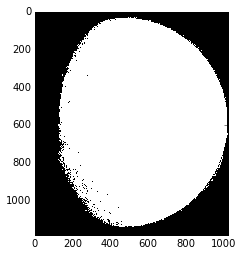
\includegraphics[scale=0.9]{moon_hist_filtered}
\caption{The sample image filtered by pixels with grayscale value > 0.01.}
\end{figure}
\\
This approach has many limitations. Our sample image conveniently focuses only on the moon and contains a nearly-perfect black background. Other images may contain any number of other objects and may not even contain the moon at all. Indeed, this method only works well in this well-defined case of a cropped image of a moon against a dark background.
\subsubsection*{Otsu's Method}
Otsu's method may give us more flexibility and requires less manual effort in selecting a threshold since it does that for us. We take two approaches: the first is a global threshold which takes into account two classes of pixels across the whole image, and the second is a local threshold (multi-Otsu thresholding) which takes into account many classes of pixels in the image by moving over portions of a certain radius. 
\begin{figure}[h]
\centering
\subfigure[Global Otsu Threshold]{\label{fig:a}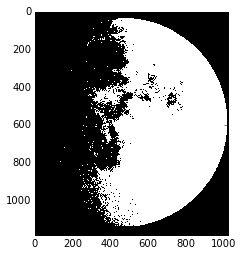
\includegraphics[scale=0.6]{global_otsu_moon}}
\subfigure[Local Otsu Threshold]{\label{fig:b}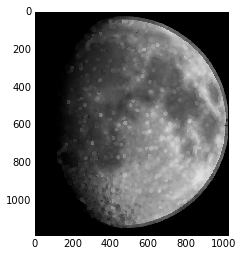
\includegraphics[scale=0.6]{local_otsu_moon_classes}}
\subfigure[Binary Local Otsu Threshold]{\label{fig:c}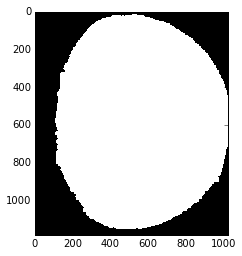
\includegraphics[scale=0.6]{local_otsu_moon}}
\caption{Otsu's method thresholds.}
\end{figure}
\\
The local threshold (Figure 4(b)) is more discerning than the global one (Figure 4(a)), which can be more or less helpful depending on the particular use case. In this case, we use a local radius of 10 pixels. Here, it's helpful because it allows us to include gray areas near the lunar terminator that the global threshold leaves out. When we count these gray areas in our illuminated area, we get a nice outline of the current phase of the moon (Figure 4(c)).
\subsubsection*{Canny Edge Detection}
Canny edge detection performs surprisingly poorly in this case. Using a low standard deviation parameter of $1/2$ to be more forgiving, this method fails to detect a single obvious "edge" to the moon, likely because the texture of the moon does not make for an obvious object. 
\begin{figure}[h]
\centering
\subfigure[Canny Edges]{\label{fig:a}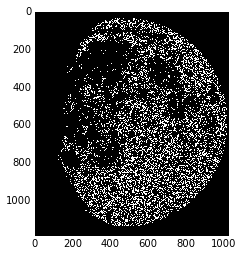
\includegraphics[scale=0.9]{canny_edges}}
\subfigure[Filled Canny Edges]{\label{fig:b}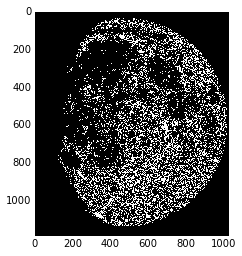
\includegraphics[scale=0.9]{canny_filled}}
\caption{Canny edges.}
\end{figure}
\\
Instead, many points are selected as edges (Figure 5(a)). This makes it difficult to easily fill a shape, since there is no clear-cut border around the moon, but instead many small patches of potential edges. This leaves us with a poorly-filled shape (Figure 5(b)). One way to remedy this is to be more liberal in filling the "edges", or don't even consider the output to be edges, but rather some mask of illuminated area, and fill all gaps within it (as if it was a continuous edge).
\pagebreak
\subsubsection*{Region-based Segmentation}
We implement region-based segmentation by first creating an elevation map using the Sobel operator, which emphasizes the sharp gradient along the edge of the Moon. We then select regions in and out of the Moon and fill similar pixels those regions until we reach the sharp gradients.
\begin{figure}[h]
\centering
\subfigure[Elevation Map]{\label{fig:a}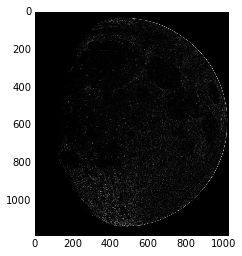
\includegraphics[scale=0.6]{elevation_map}}
\subfigure[Filled Region]{\label{fig:b}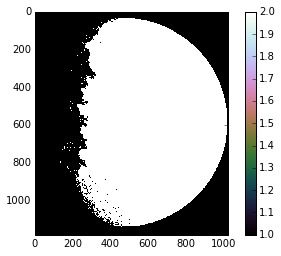
\includegraphics[scale=0.6]{region_segmentation}}
\caption{Region-based segmentation.}
\end{figure}
\\
The sharp delta at the edge of the moon serves this method well, allowing it to fill a relatively accurate region of the illuminated moon. It does well in deciding when to stop filling in the moon, but it is hindered slightly by the darkness of the lava beds and craters near the terminator, leaving an uneven edge.
\subsubsection*{Template-matching}
For our templates to compare to images for cross-correlation matching, we turn to NASA for images of the moon at different days throughout its cycle (Figure 7). While not precise to the minute, these templates are well-spread enough to give us good approximate coverage of most images of the moon, or at least enough detail to guess the current phase.
\begin{figure}[h]
\centering
\subfigure{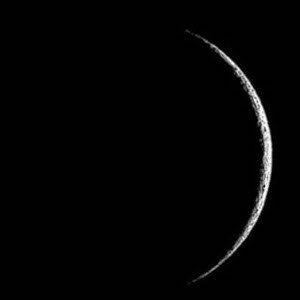
\includegraphics[scale=0.18]{../templates/moon/01}}
\subfigure{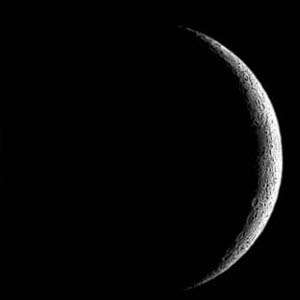
\includegraphics[scale=0.18]{../templates/moon/02}}
\subfigure{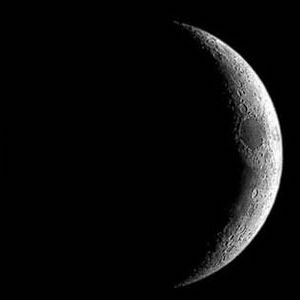
\includegraphics[scale=0.18]{../templates/moon/03}}
\subfigure{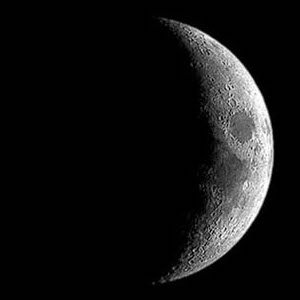
\includegraphics[scale=0.18]{../templates/moon/04}}
\subfigure{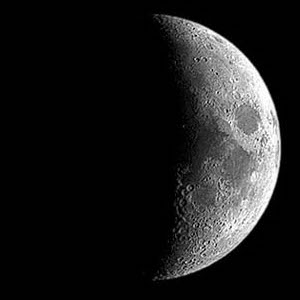
\includegraphics[scale=0.18]{../templates/moon/05}}
\subfigure{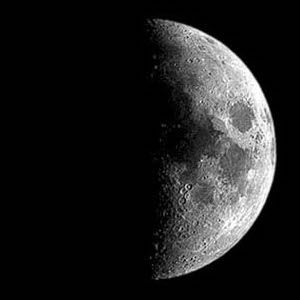
\includegraphics[scale=0.18]{../templates/moon/06}}
\subfigure{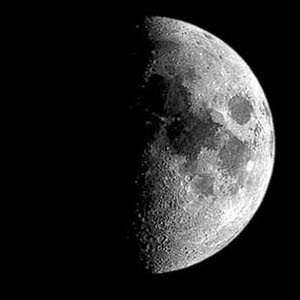
\includegraphics[scale=0.18]{../templates/moon/07}}
\subfigure{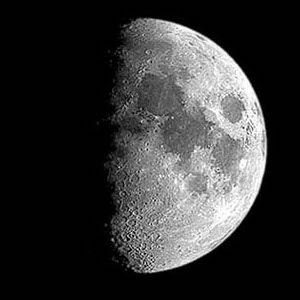
\includegraphics[scale=0.18]{../templates/moon/08}}
\subfigure{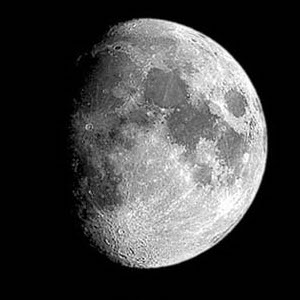
\includegraphics[scale=0.18]{../templates/moon/09}}
\subfigure{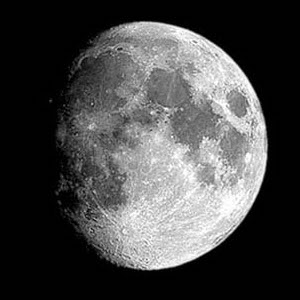
\includegraphics[scale=0.18]{../templates/moon/10}}
\subfigure{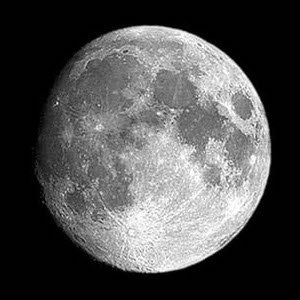
\includegraphics[scale=0.18]{../templates/moon/11}}
\subfigure{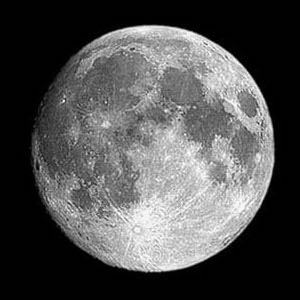
\includegraphics[scale=0.18]{../templates/moon/12}}
\subfigure{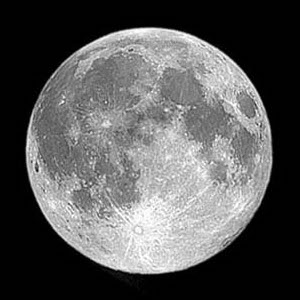
\includegraphics[scale=0.18]{../templates/moon/13}}
\subfigure{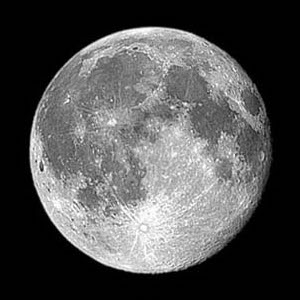
\includegraphics[scale=0.18]{../templates/moon/14}}
\subfigure{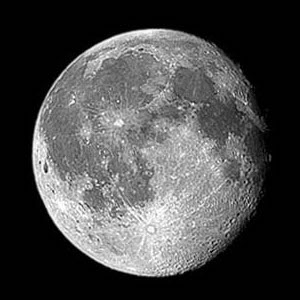
\includegraphics[scale=0.18]{../templates/moon/15}}
\subfigure{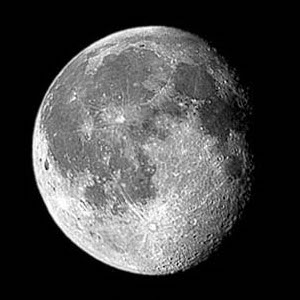
\includegraphics[scale=0.18]{../templates/moon/16}}
\subfigure{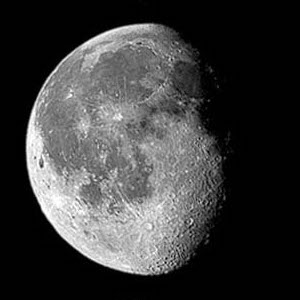
\includegraphics[scale=0.18]{../templates/moon/17}}
\subfigure{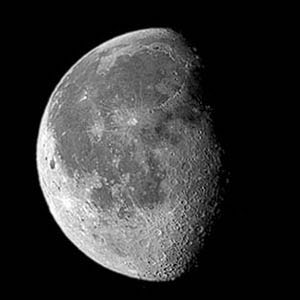
\includegraphics[scale=0.18]{../templates/moon/18}}
\subfigure{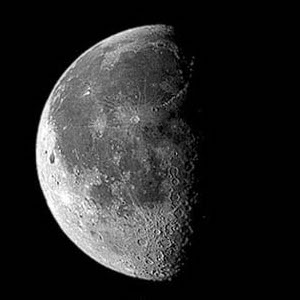
\includegraphics[scale=0.18]{../templates/moon/19}}
\subfigure{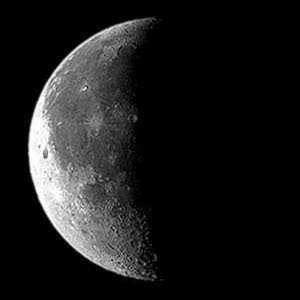
\includegraphics[scale=0.18]{../templates/moon/20}}
\subfigure{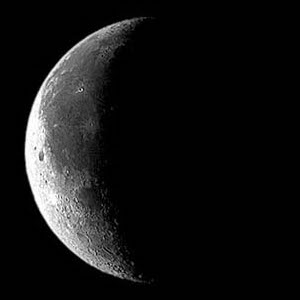
\includegraphics[scale=0.18]{../templates/moon/21}}
\subfigure{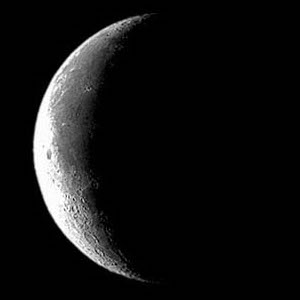
\includegraphics[scale=0.18]{../templates/moon/22}}
\subfigure{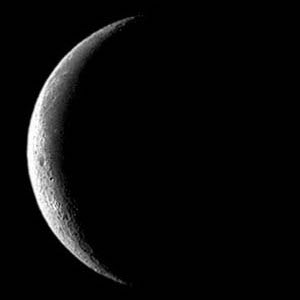
\includegraphics[scale=0.18]{../templates/moon/23}}
\caption{Templates for approximately each phase of the moon by day (via NASA).}
\end{figure}
\pagebreak
\\
Running the cross-correlation is a simple but time-consuming process because of the brute-force nature of our approach. For every AstroBin image, we cycle through every template and decide which of the 23 templates gives us the highest match. The highest match is decided simply by which correlation image has the maximum correlation value (on a scale from -1 to 1).
\begin{figure}[h]
\centering
\subfigure[Sample Moon]{\label{fig:a}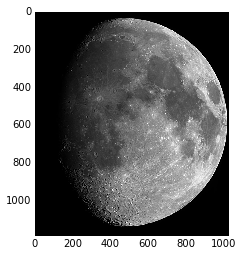
\includegraphics[scale=0.6]{sample_moon}}
\subfigure[Cross-correlation]{\label{fig:b}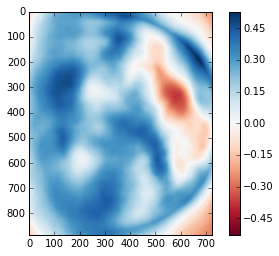
\includegraphics[scale=0.6]{crosscorrelation}}
\subfigure[Selected Match]{\label{fig:b}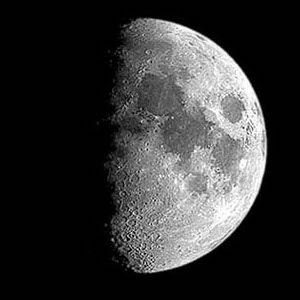
\includegraphics[scale=0.45]{template_match}}
\caption{The result of template-matching our sample moon against NASA images.}
\end{figure}
\\
Though the template-matching was run on many images with reasonable accuracy, we select the cross-correlation plot (Figure 8(b)) of our sample image (Figure 8(a)) and the best match (Figure 8(c)) to analyze the effectiveness of this approach. Although the template which was selected as the best match does indeed reflect the waxing gibbous phase of the sample image, it does not appear to be the best match among the templates upon visual inspection, since the template match is closer to a quarter moon than some of the other templates are to the waxing gibbous moon. Inspection of the cross-correlation plot shows strong correlation among the lava beds and craters in the illuminated portion of the moon, but it also shows strong correlation in the dark edges of the image. This is a huge issue with this approach -- correlation must be considered for the moon phase and not for background noise. Our algorithm selects the max, and if the portion of the cross-correlation that matched the template best happened to be the night sky, that image would be chose. We set a tunable threshold parameter to reject any images with correlation below 0.5, but that does not account for the possible false-positive matching of the night sky. Different hueristics can be used to judge which template is the best match. For example, taking the mean of the cross-correlation may be a safer approach. Additionally, looking at sequences of multiple templates and choosing the strongest match in a sequence of strong matches may also help account for any false-positives. This approach also gives us confidence in the general range of the Moon's phase.
\subsection*{Challenges and Future Directions}
Each of the approaches taken above has its own strengths and weaknesses, as previously discussed. It is these strengths and weaknesses combined that pose a challenge and an opportunity for any scientist looking to make use of astronomical data mined from amateur astronomers on the Internet. This project set out to create a method of generalized crowd-sourced timelapses for any object in the solar system, but we were quickly confronted with the harsh reality of dealing with chaotic data. All of these methods on their own fail to handle all cases, but perhaps some combination of methods can be more effective in handling most cases. For example, we can use template matching or a trained classifier to reject images without our object of interest, and identify and crop only the relevant portions of images that do contain the object. This creates a more controlled case where the thresholding and segmentation methods described above can operate more effectively in extracting information from the image. We did not even have the opportunity to confront the issue of aligning, stacking, and combining images of differing quality to create animations. In the case of images with stars in the background, Astrometry.net can be used to easily align images, but in cases where we can rely only on other computer vision methods, more creativity is necessary to ensure quality alignment.
\section*{Conclusion}
The Internet presents a huge repository of astronomical data, but we must overcome the challenge of cleaning and organizing that data to make meaningful use of it. Though no one approach described above succeeded in extracting meaningful information from most of the images we downloaded from AstroBin, we have outlined approaches which can potentially be more effective and generalizable when combined. The state of computer vision is improving rapidly, and machine learning techniques such as neural networks are becoming increasingly powerful in identifying and classifying information in images. Training classifiers could be incredibly useful in the process of cleaning and classifying data for further analysis by less flexible but otherwise reliable algorithms. Combined with metadata and user-inputted data on websites such as AstroBin, the Internet has presented us with a valuable source of scientific data. Now that we've observed its potential, the challenge lies in developing our statistical and computational knowledge in seeing that potential through. That is scientific potential even a computer can see.
\end{document}